\subsection*{Hovedmenu} \label{sec:MVCHovedmenu}
Hovedmenuen er den primære grænseflade, der inddeles i en boundary samt en dertilhørende controller. Disse fremgår af \autoref{fig:Designhovedmenu}.

\begin{figure} [H]
\centering
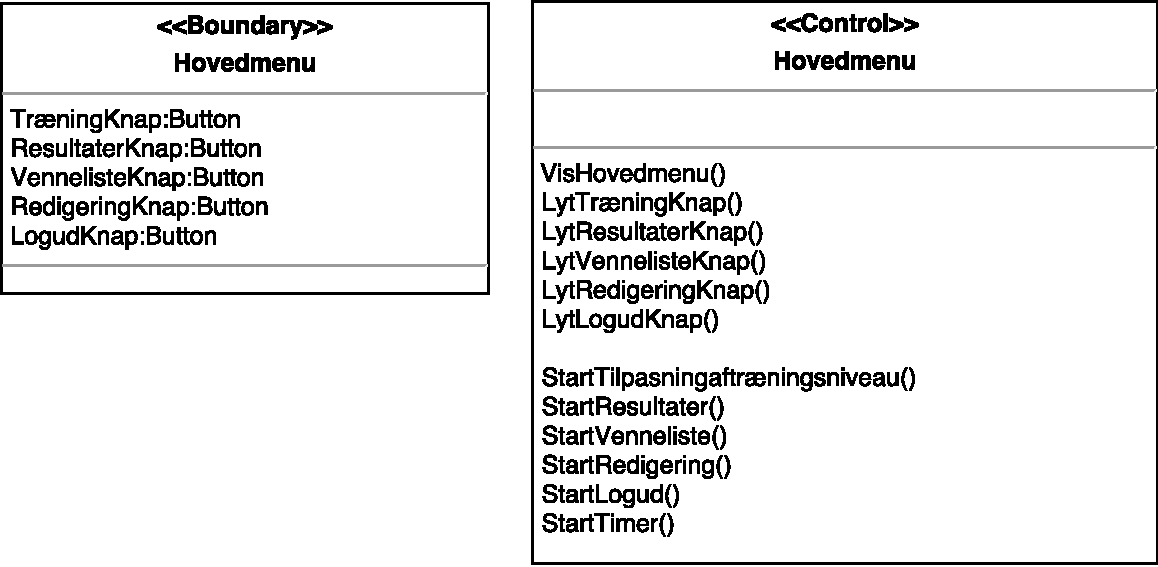
\includegraphics[width=0.9\textwidth]{figures/MVC/MVCHovedmenu}
\caption{Designklasser for hovedmenu.}
\label{fig:Designhovedmenu}
\end{figure}

\noindent
Grænsefladen for \textit{Hovedmenu} skal tillade adgang til de forskellige funktionaliteter af app’en, herunder skal det være muligt at tilgå træning, resultater, venneliste, redigering samt log ud. Funktionaliteterne tilgås via tilhørende knapper af typen button. 

Controlleren til grænsefladen viser layoutet for hovedmenuen og lytter derudover til de forskellige knapper. Et sekvensdiagram hertil er udarbejdet, hvilket fremgår af \autoref{sec:SEKHovedmenu}

\begin{figure} [H]
\centering
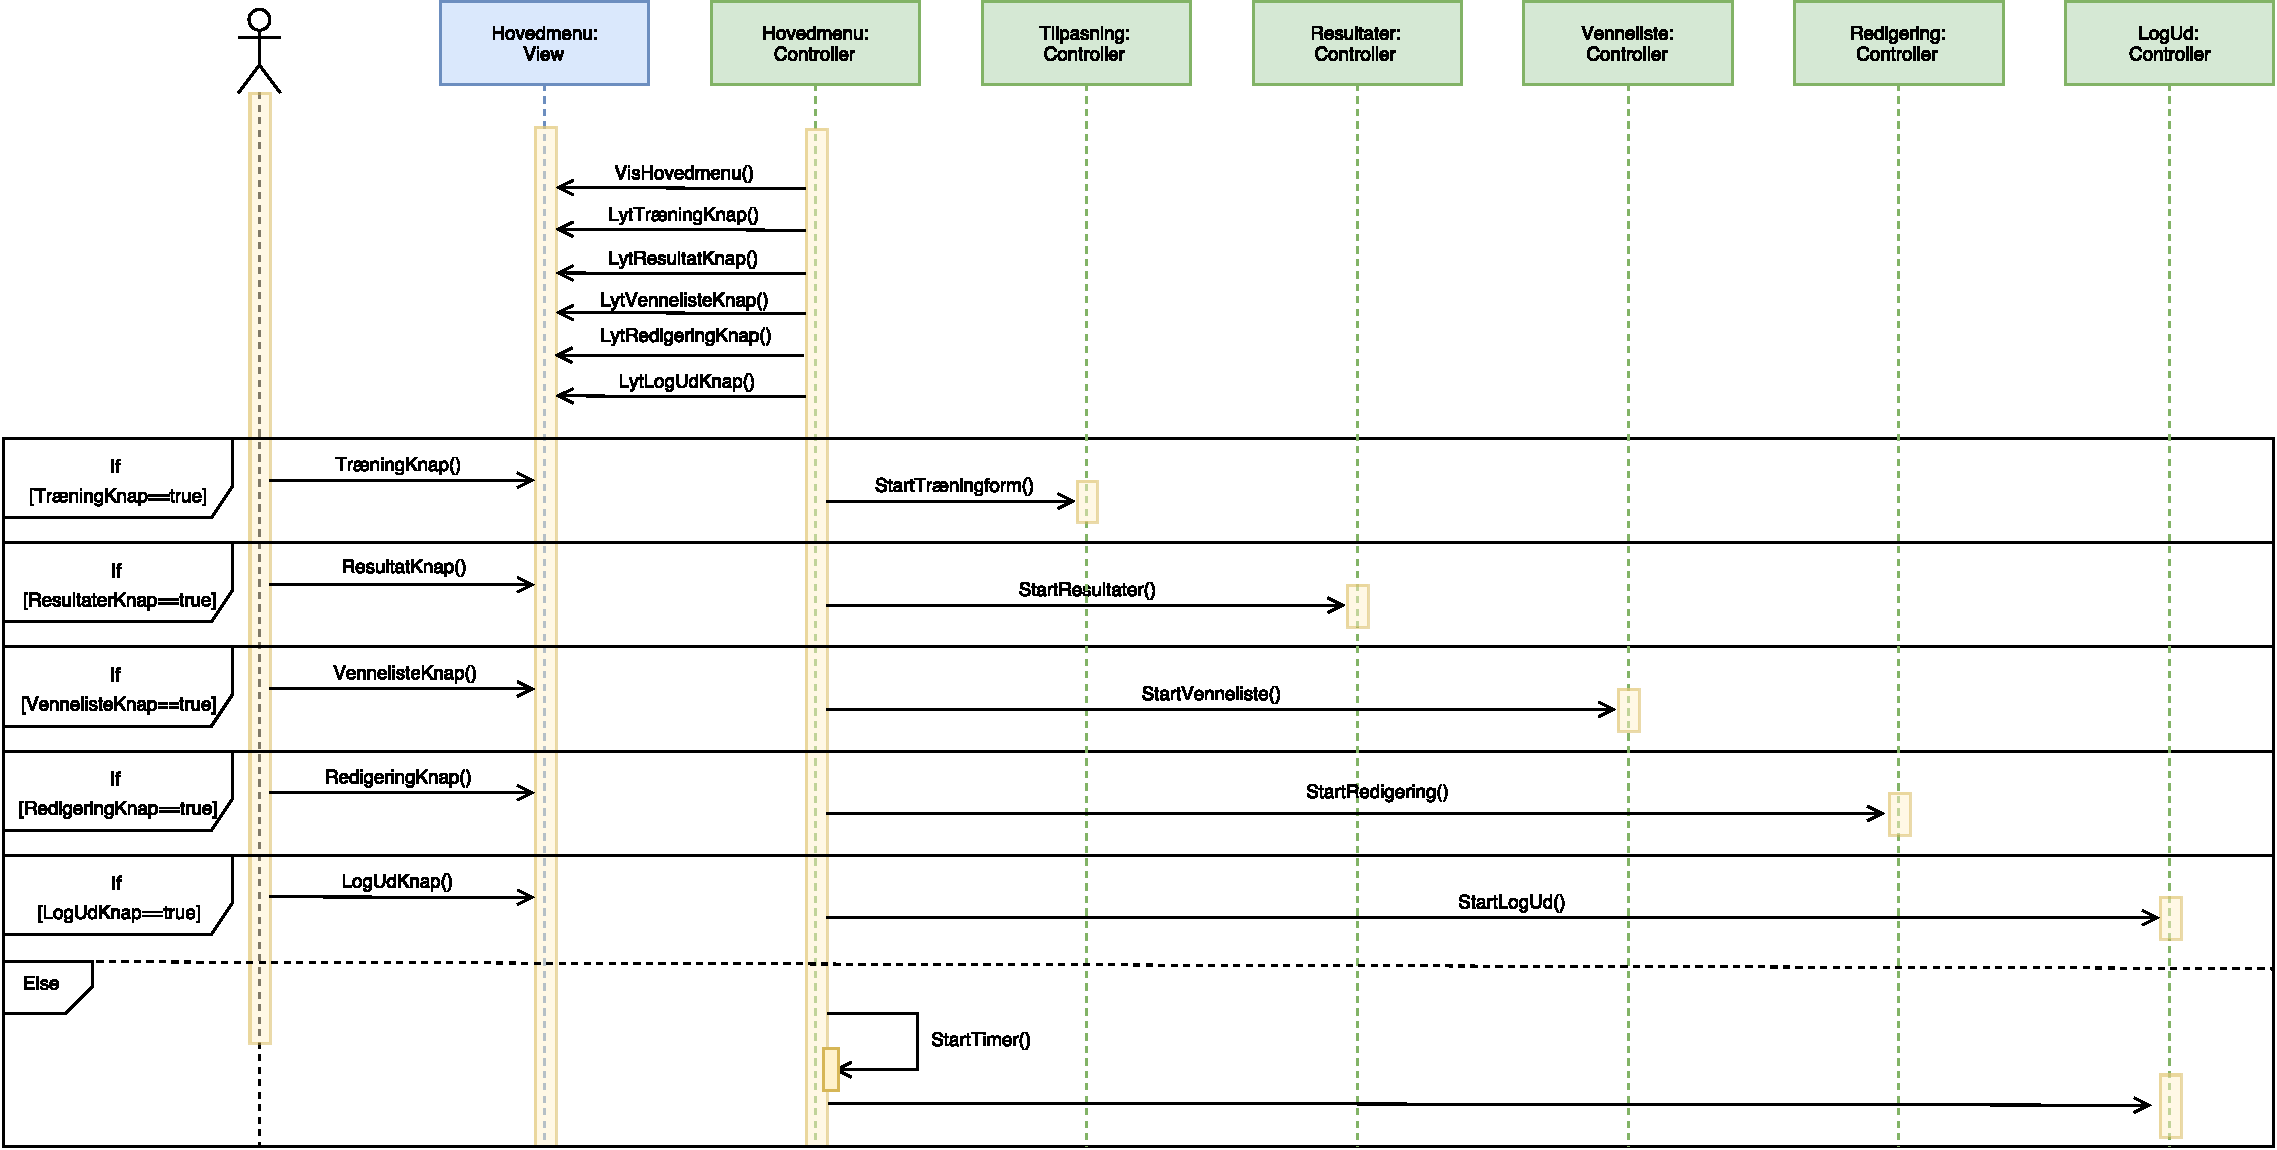
\includegraphics[width=0.9\textwidth]{figures/Sek/SEKHovedmenu}
\caption{Sekvensdiagram for hovedmenu.}
\label{fig:SEKHovedmenu}
\end{figure}

Det fremgår af sekvensdiagrammet, at der er opstillet forskellige if-løkker, som viser sekvensen for hver sin knap. Når brugeren angiver sin ønskede funktion, henvises systemet til den dertilhørende controller. Hvis ingen af de opsatte knapper angives, forbliver grænsefladen for \textit{Hovedmenuen} vist. 